\documentclass[a4paper,12pt]{article}
\usepackage[utf8]{inputenc}
\usepackage[T1]{fontenc}
\usepackage[french]{babel}
\usepackage{libertine}
\usepackage{hyperref}
\usepackage{xcolor}
\usepackage{natbib}
\usepackage{graphicx}

\hypersetup{
  colorlinks=true,
  citecolor=black!60!blue,
  linkcolor=black!40!red,
}\frac{•}{•}


\title{Détermination du caractère anaphorique du pronom personnel \og{}\textit{il}\fg{}}
\author{Agathe \textsc{Mollé}}
\date{}

\begin{document}

\maketitle

\begin{abstract}

\end{abstract}


\renewcommand\abstractname{Abstract}
\begin{abstract}

\end{abstract}


\paragraph{}

\renewcommand\abstractname{Mots-clés}
\begin{abstract}
Co-référence, Apprentissage automatique, Pronom anaphorique, Pronom impersonnel, Résolution d'anaphores
\end{abstract}

\renewcommand\abstractname{Keywords}
\begin{abstract}
Co-reference, Machine Learning, Anaphoric pronoun, Expletive pronoun, Anaphora resolution
\end{abstract}

\color{gray}

\section*{Introduction}

Les anaphores sont des expressions qui permettent de désigner des entités dans les textes (\og \textit{il} \fg{}, \og \textit{cette maison} \fg{}). Une expression anaphorique n'a de sens que si l'on dispose de son antécédent, autrement dit d'une expression précédente désignant la même entité. Par exemple, dans la phrase \og \textit{Vendredi, \textbf{M. Edmond Maire} a réuni la presse pour apporter \underline{\textbf{son}} soutien à \underline{\textbf{sa}} fédération des cheminots} \fg{}, les expressions anaphoriques \og \textit{son} \fg{} et \og \textit{sa} \fg{} réfèrent à la même entité que leur antécédent \og \textit{M. Edmond Maire} \fg{}.

La résolution d'anaphores consiste à déterminer quel est l'antécédent (ou les antécédents) de l'expression anaphorique. C'est une problématique fondamentale partagée par divers domaines du Traitement Automatique des Langues.

\paragraph{}
L'une des étapes de cette problématique est la détermination de l'aspect co-référentiel d'une expression.
Dans ce contexte, nous nous intéressons aux pronoms car ils ont pour avantage d'être fréquents et facilement identifiables \citep{danlos-ilimp-taln2005}, et plus particulièrement au pronom personnel de la 3\up{ème} personne du singulier, masculin : \og{}\textit{il}\fg{}. 
En effet, selon les cas, celui-ci peut s'avérer : 
\begin{itemize}
 \item co-référentiel (anaphorique)\\ \og{}\textit{\underline{il} ne pouvait entrer ainsi dans un conflit ouvert}\fg{}
 \item non-coréférentiel (impersonnel)\\ \og{}\textit{\underline{il} est temps de mettre un terme à la grève}\fg{}
\end{itemize}

\paragraph{}
Il existe actuellement plusieurs techniques traitant du pronom personnel \og{}\textit{it}\fg{} en anglais.
Certaines sont à base de règles lexico-syntaxiques \citep{Lappin-1994-APA-203987.203989}, d'autres à base d'apprentissage \citep{Li-2009-IPU-1622716.1622726} ou d'observations statistiques \citep{Bergsma-11}.


Pour le français, il n'existe qu'un outil à base de règles \citep{danlos-ilimp-taln2005}. Celui-ci obtient de très bons résultats, mais les outils à base de règles manquent généralement de robustesse. Il est en effet difficile d'énumérer de manière exhaustive toutes les constructions impersonnelles. Par ailleurs, cet outil n'effectue pas de désambiguïsation morpho-syntaxique lors de son prétraitement, il souffre donc d'erreurs liées à l'absence d'analyse syntaxique.

\paragraph{}
L'objectif de notre travail est d'établir un système déterminant le caractère anaphorique du \og{}\textit{il}\fg{} français. L'approche à base de règles est abandonnée au profit d'une approche à base d'apprentissage automatique supervisé. Cette tâche peut en effet être considérée comme une tâche de classification : en décrivant chaque instance de \og \textit{il} \fg{} par un jeu de traits appropriés, on peut ensuite prédire l'étiquette d'une nouvelle instance, étant donné son vecteur de traits. On peut aussi chercher à définir la tâche comme un problème d'étiquetage de séquences (\emph{sequence labeling}), de par sa sensibilité au contexte local. Dans le cas du pronom \og \textit{il} \fg{}, nous n'avons pas affaire à des séquences proprement dites puisqu'il n'y a qu'un seul élément à étudier. Cependant, l'approche par étiquetage de séquences se justifie par la volonté d'étendre ces travaux à la détermination du caractère anaphorique des descriptions définies (celles-ci étant des séquences comme\og \textit{l'homme} \fg{}, \og \textit{la maison de Paul} \fg{}, \ldots).

\paragraph{}
Notre tâche pouvant être définie selon ces deux approches, il convient de les expérimenter toutes deux. Lors de la planification d'expériences, il s'est avéré plus simple de réaliser l'expérience avec l'étiqueteur de séquences\footnote{\samepage L'expérience avec l'étiqueteur de séquences consistait en une extension d'un TP réalisé sur la reconnaissance d'entités nommées}.
En l'état de notre avancement, nous ne rapportons pour l'instant que les deux expériences à base d'étiquetage de séquences.
Nous expérimentons en effet deux jeux de traits pour caractériser les pronoms et leur contexte.
La première expérience consiste à utiliser les traits classiques de la détection de segments syntaxiques pour le français. Pour la deuxième, nous dégageons de nouveaux traits par observation du corpus de développement (un dixième du corpus total) et par recensement de traits mentionnés dans la littérature.

Pour réaliser nos expériences, nous disposons du corpus \cite{tutin-hal-00373327}, lequel est seulement annoté avec les expressions anaphoriques. Nous indiquerons dans la section~\ref{annotation-imp} comment nous avons procédé pour constituer un corpus avec des instances de chaque classe.

\paragraph{}
La section~\ref{etat-art} décrit dans un premier temps les travaux existants sur lesquels nous nous sommes appuyés. La section~\ref{corpus} présente notre corpus de travail, la section~\ref{approche-traits} les traits que nous avons recensé et que nous utilisons pour nos expérimentations.
La section~\ref{xp} présente le déroulement des expériences que nous avons réalisé sur ce corpus.
Enfin, en section~\ref{resultats}, nous détaillons les résultats obtenus ainsi qu'une discussion sur le travail effectué et sur ce qu'il pourrait être intéressant d'exploiter à l'avenir.

\color{black}

\section{État de l'art}
\label{etat-art}

\subsection{Caractère impersonnel du \og \textit{il} \fg{}}

\color{gray}

Pour résoudre cette tâche, nous nous sommes appuyés sur les seuls travaux à notre connaissance en français \citep{danlos-ilimp-taln2005} et sur l'un des plus récents pour l'anglais \citep{Bergsma-11}.

\paragraph{}
En effet, les travaux de \citet{Lappin-1994-APA-203987.203989} utilisent des règles qui s'appuient sur la structure syntaxique de l'anglais, donc ne sont pas aisément portables au français. De même, les autres approches par classification ont été mises de côté, car les traits apportés aux classifieurs dépendent eux aussi de règles grammaticales anglaises.

\paragraph{}
L'approche à base de règles développée pour le français est l'outil ILIMP, conçu pour classer les occurrences du pronom \og{}\textit{il}\fg{} selon si elles sont anaphoriques ou impersonnelles \citep{danlos-ilimp-taln2005}. Cet outil travaille sur des textes bruts, non annotés.

Le travail de L. \citeauthor{danlos-ilimp-taln2005} se définit en deux temps : la première démarche conduit à l'élaboration de règles, puis la seconde amène à la reconnaissance des constructions impersonnelles ou anaphoriques en appliquant les règles en question.

Pour élaborer les règles, \citeauthor{danlos-ilimp-taln2005} observe les propriétés lexicales et syntaxiques des constructions impersonnelles, et plus particulièrement de leur tête lexicale. Elle s'appuie sur le lexique-grammaire du français\footnote{http://infolingu.univ-mlv.fr/} \citep{gross-halshs-00278309,leclere-hal-00192888}
 qui décrit l'ensemble des têtes lexicales des phrases simples du français, avec leurs arguments syntaxiques et les alternances possibles.
Elle définit alors une liste de verbes, adjectifs et expressions caractérisant des constructions impersonnelles, qu'elle divise d'ailleurs en deux catégories : les constructions intrinsèquement impersonnelles, qui ne peuvent avoir comme sujet que \og \textit{il} \fg{}, et les constructions impersonnelles à sujet profond extraposé (sujet phrastique ou nominal). On peut distinguer par exemple les verbes météorologiques qui ancrent des constructions intrinsèquement impersonnelles (\og \textit{Il pleut} \fg{}), ou alors des adjectifs tels \og \textit{probable} \fg{} qui traduisent des constructions impersonnelles à sujet (phrastique) profond extraposé (\og \textit{Il est probable que Fred viendra} \fg{}).

Pour chaque construction impersonnelle, il se trouve que le contexte gauche de la tête lexicale, même s'il est complexe, est analysable sans trop de difficultés.
Par exemple, on peut rencontrer les constructions suivantes\footnote{Les exemples mentionnés sont tirés de l'article \textit{ILIMP : Outil pour repérer les occurrences du pronom impersonnel il} par \citet{danlos-ilimp-taln2005}} :

\og{}\textit{\textbf{Il est} difficile de résoudre ce problème.}\fg{}

\og{}\textit{\textbf{Il peut lui paraître très} difficile de résoudre ce problème.}\fg{}

\og{}\textit{\textbf{Il ne s'est pas avéré} difficile de résoudre ce problème.}\fg{}

Dans ces 3 cas, la tête lexicale est l'adjectif \og \textit{difficile} \fg{} mais le contexte gauche varie. Il s'agit alors de répertorier tous les cas possibles et de les intégrer dans les règles, opération minutieuse mais qui ne pose pas de réel problème.

A l'inverse, c'est le contexte droit qui peut poser des ambiguïtés. Celles-ci peuvent être d'ordre syntaxique (une séquence peut recevoir plusieurs analyses syntaxiques), d'ordre lexical (par exemple \og{}\textit{Il est certain que Fred viendra.}\fg{} peut être à la fois anaphorique et impersonnelle) ou alors être dûes à des constructions impersonnelles qui ne diffèrent en surface que de façon très subtile par rapport à des constructions personnelles (\og{}\textit{Il reste la valise du chef}\fg{} (impersonnelle) / \og{}\textit{Il reste la priorité du chef (le chômage)}\fg{} (anaphorique)).

Pour éviter d'avoir trop de constructions considérées comme \og ambiguës \fg{}, \citeauthor{danlos-ilimp-taln2005} va avoir recours à des heuristiques établies à partir d'études quantitatives ou de ses intuitions linguistiques. Par exemple, pour une construction donnée, si on analyse plus fréquemment les phrases comme impersonnelles dans les corpus, alors cette construction sera par la suite considérée comme telle.

\paragraph*{}
Afin de les incorporer à ILIMP, ces règles sont traduites en patrons linguistiques grâce à l'outil UNITEX\footnote{http://www-igm.univ-mlv.fr/~unitex/\#}. Par exemple, une construction typiquement impersonnelle est le verbe \og \textit{être} \fg{} à la 3ème personne du singulier, suivi d'un adjectif du lexique préalablement défini (il est ici la tête lexicale), suivi de la proposition \og \textit{de} \fg{} et d'un verbe à l'infinitif, on écrit alors le patron suivant :

\verb!Il[IMP] <être.V:3s> <Adj1:ms> de <V:W>!

Ce patron correspond ainsi à des phrases comme :

\og{}\textit{Il est difficile de résoudre ce problème.}\fg{}

UNITEX prend en entrée des données brutes, et les prétraite en effectuant une tokénisation, et en attribuant à chaque token toutes les propriétés morpho-syntaxiques et flexionnelles que celui-ci peut avoir (obtenues grâce au dictionnaire DELAF \citet{courtois}).

Les données prétraitées et les patrons écrits, il s'agit maintenant de décorer chaque occurrence de \og \textit{il} \fg{} de la balise adéquate, à savoir \verb![IMP]! (impersonnelle),  \verb![ANA]! (anaphorique) ou \verb![AMB]! (ambiguë).

Pour ce faire, toutes les occurrences de \og \textit{il} \fg{} reçoivent par défaut la balise \verb![ANA]!. A chaque fois que la construction correspond à un des patrons prédéfinis, celle-ci devient alors \verb![IMP]!. Si le cas est ambigu, et que les heuristiques n'ont pas suffi à déterminer le caractère impersonnel de la construction, la balise \verb![AMB]! est alors employée.

\paragraph*{}
Pour évaluer ILIMP, le corpus utilisé est \emph{Le Monde}, comportant 3 782 613 tokens, dont 13 611 occurrences de \og{}\textit{il}\fg{}, celles-ci ayant été annotées à la main. Il ressort de cette évaluation un taux de précision de 97.5\%. La plupart des erreurs obtenues sont des balises \verb![ANA]! à la place de \verb![IMP]! car \verb![ANA]! est la balise par défaut, et les règles utilisées n'ont pas couvert tous les cas. Par exemple, l'inversion du sujet n'a pas été correctement traitée, le lexique des adjectifs impersonnels est incomplet ou encore l'impasse a été faite sur la coordination.
Il y a peu d'erreurs \verb![IMP]! à la place de \verb![ANA]! malgré les heuristiques brutales.
Un étiquetage morpho-syntaxique aurait pu éviter certaines erreurs de prédiction.

\paragraph{}
L'approche pour l'anglais proposée par \citet{Bergsma-11}, va allier l'apprentissage automatique supervisé et des observations statistiques.
Ce système (\textit{NADA : Non-Anaphoric Detection Algorithm}) prend en entrée des données tokénisées et détecte les occurences de \og{}\textit{it}\fg{} non-coréférentielles. Les données en question n'ont pas été analysées morpho-syntaxiquement, car le postulat est fait que l'ambiguïté repose sur la présence d'entités lexicales spécifiques, et non sur les informations morpho-syntaxiques.
Par exemple\footnote{Les exemples mentionnés sont tirés de l'article \textit{NADA : A robust system for non-referential pronoun detection} par \citet{Bergsma-11}} :

\og{} \textit{It is \textbf{able} to maintain a stable price.} \fg{}

\og{} \textit{It is \textbf{important} to maintain a stable price.} \fg{}
\setcitestyle{numbers,square}\\
sont composés de la même séquence d'étiquettes syntaxiques, seul l'adjectif les différencie : \textit{able}/\textit{important}.

Deux types de traits sont alors apportés au classifieur : des traits lexicaux-syntaxiques, mais aussi des statistiques tirées du corpus n-gramme de Google \citep{google-ngram}. Le classifieur est fondé sur un modèle de régression. Les traits lexicaux sont extraits sur la phrase entière. Il y a par exemple la présence d'autres formes du pronom personnel (\textit{its}/\textit{itself}), la présence d'acronymes, de prépositions juste avant le nom, de certains tokens prédéfinis tels \og{}\textit{that}\fg{} ou \og{}\textit{says}\fg{} après le pronom, etc.
Les traits statistiques sont établis grâce à l'énorme banque de données fournie par Google. En effet, pour chaque 4-gramme contenant le pronom \og{}\textit{it}\fg{}, on va établir un patron (le \og{}\textit{it}\fg{} est remplacé par un \og{}\textit{\_}\fg{}) et observer dans les données si d'autres mots remplissent ce patron, ou si seulement le cas de figure avec \og{}\textit{it}\fg{} a été rencontré. Par exemple, si on extrait \og{}\textit{it is able to}\fg{}, on va rechercher toutes les occurences de la forme \og{}\textit{\_ is able to}\fg{}.
Les résultats obtenus permettent d'ajouter un trait (un poids) dans le classifieur.
Seulement, ce corpus étant gigantesque, il a fallu le compresser au maximum. Pour ce faire, diverses techniques ont été utilisées : ne récupérer que les 4-grammes, uniquement ceux contenant \og{}\textit{it}\fg{}, \og{}\textit{they}\fg{} ou \og{}\textit{them}\fg{}, tronquer les mots à 4 caractères, les encoder, ne retenir que les changements d'un 4-gramme à l'autre, etc.

NADA a été évalué sur les corpus BBN \cite{BBN}, WSJ-2 (tiré du Penn Treebank \cite{Marcus-1993-BLA-972470.972475}) et ItBank \cite{Bergsma08distributionalidentification}. Les résultats sont similaires pour les 3 corpus (entre 85,1\% et 86,2\%). Par comparaison, l'évaluation a aussi été réalisée avec seulement les traits lexicaux et seulement les traits statistiques, obtenant de moins bons résultats indépendamment (en moyenne 80\% pour les traits lexicaux et 83,5\% pour les traits statistiques).

Les approches par classification obtiennent à l'heure actuelle les meilleurs résultats pour le cas du pronom \og \textit{it} \fg{} anglais, c'est pourquoi nous cherchons à les adapter aux textes français.
\setcitestyle{authoryear,round}

\color{black}



\paragraph{Résumé Li}
Tandis que de nombreux systèmes de résolution d'anaphores ignorent le problème des pronoms pléonastiques et choisissent de nettoyer leur données, (ref) considère qu'il est très important de les prendre en compte.
En effet, on dénombre entre 16\% et 50\% de pronoms impersonnels sur du texte anglais.
Ils classent le pronom \og it \fg{} selon 4 classes :
\begin{itemize}
\item les référentiels avec antécédent nominal
\item les référentiels avec antécédent phrastique
\item les pronoms qui n'ont pas d'antécédent (pléonastique) parmi lesquels on peut lister les extrapositions, les cleft (TODO trad) et les local situation (TODO trad)
\item les pronoms idiomatiques
\end{itemize}
(ref) s'intéressent au cas pléonastique (la troisième classe).

Leur système se décompose en 3 phases : le prétraitement, le filtrage syntaxique puis les requêtes sur le web.
Lors du prétraitement, (ref) construisent un arbre de dépendances. (TODO détailler ?). Pour le filtrage, des patrons cherchent à reconnaître une construction météorologique ou temporelle, ainsi que les clefts et les extrapositions.
Enfin, le web est utilisé pour désambiguïser les données restantes. La question peut se poser quant à l'utilisation du web en tant que corpus, étant donné que celui-ci est mal équilibré, souffre de nombreuses erreurs et est difficile à exploiter. Cependant, (ref) affirment qu'il est pertinent par sa taille, et par sa capacité à évoluer dans le temps (nouveaux termes).

TODO : résultats




\subsection{Ressources}

\paragraph{Résumé Candito (HS)}
(ref) ont produit une analyse syntaxique statistique à la fois en constituants et en dépendances pour le Français. Leur technique consiste à s'appuyer sur un analyseur statistique en constituants puis de le convertir en dépendances typées. Ils travaillent sur le French Tree Bank (ref). Celui-ci préconise une annotation en constituants, et Candito va s'en inspirer pour définir son propre schéma d'annotation \textit{deps}. 

Pour convertir un arbre syntagmatique de type \textsc{Ftb} vers leur schéma \textit{deps}, ils vont dans un premier temps marquer automatiquement la tête de chaque constituant, en utilisant une table de propagation des têtes (ref). Cette étape permet de remonter sur chaque n\oe{}ud syntagmatique sa tête lexicale, et permet ensuite d'extraire des dépendances partielles. Une deuxième étape va renseigner de nouvelles dépendances non extraites à la première étape, à l'aide d'heuristiques. Puis une étape manuelle va permettre d'ajouter les dernières dépendances. Cette conversion a été évaluée sur une portion du corpus révisée manuellement et donne une F-mesure de plus de 98\%.

Pour réaliser l'analyse syntaxique automatique, ils adaptent la procédure de conversion. Ils ont par conséquent besoin de produire des données analogues à celles apportées en entrée à cette procédure. Pour cela, il faut pouvoir ajouter les étiquettes fonctionnelles sur les dépendants verbaux. Ils utilisent l'analyseur en constituants de Berkeley (ref). Deux approches sont possibles : une analyse intégrée (apprentissage d'une grammaire dont les symboles intègrent l'information fonctionnelle) qui dégrade les résultats, ou une analyse séquentielle (analyse en constituants dépourvus d'étiquette puis ajout des étiquettes de fonction en utilisant un modèle lexicalisé) qui sera choisie pour la suite.

La tâche d'étiquetage fonctionnel se réduit à un simple problème de classification. Chaque dépendant est représenté par un vecteur de traits qui décrit le dépendant, son contexte, et sa relation au gouverneur. L'apprentissage est réalisé suivant un modèle par maximum d'entropie (log-linéaire). Lors de l'évaluation de cet étiquetage fonctionnel, ils obtiennent une exactitude de 87.9\%.

Une seconde évaluation permet de mesurer les résultats sur la chaîne d'analyse complète et obtient une précision de 86.56\%. Une dernière évaluation leur a permis de tester leur modèle sur le corpus EASy (ref), moyennant une conversion, et donne un résultat de 66\%, comparable aux meilleurs résultats de la campagne d'évaluation EASy (65\%). Cependant, leur modèle est moins performant lors d'un changement de domaine (médical, par exemple).

\paragraph{Extraction têtes}
Pour analyser une construction, nous nous intéressons à sa tête ainsi qu'à son complément. Il aurait pu être judicieux d'utiliser un analyseur de dépendances, mais toutes les informations que celui-ci nous fournirait ne nous intéressent pas ici. Nous avons principalement besoin de reconnaître les constituants syntaxiques et de trouver leur tête. Nous utilisons l'analyseur syntaxique statistique en constituants d'OpenNLP (ref). Pour déterminer la tête de chaque constituant, nous avons recours à une table de propagation de têtes pour le français. Cette table, initialement proposée par Magerman 1995 puis améliorée par Collins pour l'anglais, a été adaptée au français par Arun & Keller. Nous en utilisons la version modifiée par Dybro-Johansen puis Djamé Seddah 2010. Cette table est composée de règles qui définissent comment chercher la tête selon le type du constituant. Par exemple, pour un groupe verbal, il faut chercher le dernier verbe du constituant.

\paragraph{Lexique-grammaire}
Le lexique-grammaire du français (Gross Leclère) décrit les structures syntaxiques élémentaires. Cette ressource est constituée de tables, chacune se présentant sous forme matricielle. Chaque ligne représente une entité lexicale, et les colonnes permettent d'identifier les propriétés définitoires propres à cette entité. Il recense notamment toutes les expressions figées contenant le pronom \og \textit{il} \fg{}. Nous pouvons considérer que si elles sont figées, ces expressions sont à caractère impersonnel. Ce lexique-grammaire recense également des verbes ou adjectifs ainsi que leurs propriétés. Ce sont les verbes qui nous intéressent particulièrement puisque le pronom \og \textit{il} \fg{} est un sujet. Pour chaque verbe recensé dans le lexique-grammaire, M. Gross et son équipe donnent un exemple d'utilisation de celui-ci. Il se trouve que si le verbe est anaphorique, le sujet de l'exemple est principalement un nom propre ou un groupe nominal. A l'inverse, les exemples des verbes impersonnels ne peuvent contenir comme sujet que le \og \textit{il} \fg{}. Nous pouvons donc extraire ces informations et lister les verbes ancrant des constructions impersonnelles.

\paragraph{Lefff}
Benoît Sagot a mis en place un lexique morphologique et syntaxique du français : Le Lefff (Lexique des Formes Fléchies du Français). C'est un lexique électronique recensant toutes les formes fléchies de la langue française, et qui présente des informations morphologiques et syntaxiques pour chacune d'entre elles. Moins riche que le lexique-grammaire, il a pour avantage d'être facilement utilisable dans les applications de Traitement Automatique du Langage.

Il recense plus de 110 000 lemmes, correspondant à plus de 520 000 entrées (formes verbales, certaines formes adjectivales et nominales, prépositions, \ldots). A chaque entrée, sont renseignées les informations syntaxiques, mais aussi des propriétés qui vont permettre d'établir un cadre de sous-catégorisation à la forme fléchie.

En 2006, B. Sangot et L. Danlos ont entreprit de l'enrichir à l'aide des informations fournies par le lexique-grammaire, en particulier pour les constructions impersonnelles et les expressions verbales figées. Danlos a ainsi repris son travail sur l'outil ILIMP et en a extrait les informations pouvant être apportées au Lefff. Le travail a été plus complexe pour le cas des expressions verbales figées, il est donc encore en cours de recherche.


\subsection{Résolution d'anaphores}

\paragraph{Résumé Bengston}
La résolution d'anaphores est la tâche consistant à grouper toutes les mentions d'une même entité dans une classe d'équivalence. Le choix des traits est crucial pour mener cette tâche à bien.

Les travaux de Bengston et Roth tentent de déterminer l'impact des traits pour la résolution d'anaphores. Ils utilisent un modèle par paires (\textit{pairwise coreference model}). Ils comparent en effet deux à deux les mentions afin de déterminer l'antécédent au plus grand score. Ils se démarquent par le postulat suivant : pour une mention non pronominale, aucun pronom n'est considéré comme antécédent candidat.

Ils ne considèrent qu'un antécédent au plus pour une mention. Pour réaliser leur corpus d'entraînement, ils utilisent les données ACE (ref). Ils choisissent pour chaque mention $m$, au sein de la classe d'équivalence, la mention la plus proche comme antécédent $a$, et cette paire $(a,m)$ est considérée comme un exemple positif. Ensuite, pour chaque mention $m$, toutes les autres mentions précédentes qui ne sont pas dans la même classe d'équivalence sont des exemples négatifs. Pour apprendre leur fonction d'appariement de coreference, ils utilisent l'algorithme du perceptron.

TODO définir tête et modifieur

Les traits se divisent en 8 catégories : le type de la mention, les relations morphologiques, des traits sémantiques, des traits de distance relative, des traits d'apprentissage , l'alignement des modifieurs, des traits de mémorisation et les types d'entité prédits.

L'évaluation est mesurée avec la F-mesure cubique et le F-score de MUC. Ils obtiennent un score de 80.8\% pour la première (1.5 de plus que l'état de l'art à l'époque) et 75.8\% pour la seconde.
L'impact des features a ensuité été évalué séparément, et il apparaît que les traits relatifs à l'apposition, au pronom relatif, aux distances et à la prédiction des types d'entités sont ceux qui apportent le plus de résultats.
L'évaluation a aussi été réalisée sur des données brutes, les têtes étant détectées avec les chunks et les extensions par apprentissage automatique. Le score est alors de 78.24\%.

\paragraph{Résumé Soon}
Les travaux de (ref) se sont portés sur la résolution de la coréférence pour les syntagmes nominaux. En effet, ils ne se réduisent pas aux pronoms ou à certains types d'entité, mais prennent en considération l'ensemble des groupes nominaux. Ils ont employé une approche à base d'apprentissage automatique, qui ne nécessite pas un corpus gigantesque.

Dans un premier temps, ils déterminent tous les markables (todo) à l'aide d'une cha\^ine de traitement linguistique. Ils génèrent ensuite leurs exemples d'entra\^inement (paires de markables, positives ou négatives) sous forme de vecteurs de traits. Gr\^ace à ces exemples, ils peuvent entra\^iner leur classifieur. Pour tester un nouveau document, ils détectent tous les markables, et les paires possibles sont présentées au classifieur.

La cha\^ine de traitement linguistique leur permettant de déterminer des markables à partir de texte brut se décompose en 7 étapes : la tokénisation et la segmentation en phrases, le traitement morphologique, l'étiquetage morpho-syntaxique, l'identification des syntagmes nominaux, la reconnaissance d'entités nommées, l'extraction de groupes nominaux imbriqués, et la détermination de la classe sémantique. Cette cha\^ine a été évaluée et il en ressort 85\% de markables correctement identifiés.

Pour établir leurs vecteurs de traits, (ref) observent la distance entre les deux markables (l'anaphore \textit{j} et l'antécédent potentiel \textit{i}), si \textit{i} est un pronom, si \textit{j} en est un, si ils sont identiques (en excluant l'article ou le pronom démonstratif), si le syntagme nominal est défini ou démonstratif, si leur nombre ou genre est le m\^eme, ainsi que leur classe sémantique (ou du moins si l'une est parente de l'autre), si tous les deux sont des noms propres, si l'un est un alias de l'autre (par exemple un acronyme, ou si deux entités \textit{Personne} ont le m\^eme nom de famille), et enfin si c'est une apposition.

Les exemples d'entra\^inement positifs sont déterminés comme suit : pour une cha\^ine de coréférence donnée, ils prennent les paires de syntagmes nominaux adjacents. Par exemple, pour la cha\^ine A1--A2--A3, les paires positives sont A1--A2 et A2--A3. Dans une paire, le premier groupe nominal est l'antécédent et le second l'anaphore. Pour générer les exemples négatifs, ils cherchent les autres markables se trouvant entre une anaphore et son antécédent. Par exemple, si l'on s'intéresse à la paire positive A1--A2, et que l'on rencontre dans le texte les markables A1, a, b et A2 dans cet ordre-là, on considère que les paires a--A2 et b--A2 sont négatives.

Les exemples d'entra\^inement extraits sous forme de vecteurs de traits, (ref) utilisent l'algorithme C5, un arbre de décision, pour construire leur classifieur.

Pour un nouveau document de test, ils détectent dans un premier temps tous les markables possibles. Chaque markable est considéré comme une anaphore et pour chacun, tous les markables précédents sont considérés comme antécédents possibles (sauf pour le cas des markables imbriqués). Pour chaque paire (antécédent potentiel--anaphore), on établit un vecteur de traits et le classifieur détermine si elle est succeptible d'\^etre positive. Pour une anaphore donnée, c'est le markable positif le plus proche qui est considéré comme antécédent.

Ce modèle a été évalué sur les corpus issus de MUC6 et MUC7 et obtient des F-mesures atteignant les 60\%. Ces résultats sont comparables aux performances obtenues par les approches qui ne sont pas à base d'apprentissage automatique.

\paragraph{Résumé BART}
(ref) ont développé un outil modulaire permettant de mettre en place facilement des systèmes de résolution de coréférence : BART (\textit{Baltimore Anaphora Resolution Toolkit}).
Il a été conçu afin de faciliter la recherche dans le domaine de la résolution de coréférence, il est ainsi possible de tester séparément différent modèles de prétraitement, de résolution de coréférence mais aussi de traits spécifiques à cette tâche.
Implémenté en Java, il s'appuie sur le système EMLR développé par Ponzetto et Strubes (ref) et incorpore des idées provenant du système Guitar (Poesio ref), et des travaux de Versley (ref) et Yang et al (ref).
Cet outil a été testé avec certains modèles existants, notamment les analyseurs ..... (refs, utile de tous les citer ?), ainsi que les modèles proposés par Soon et al. et Yang et al. pour résoudre ce problème de coréférence.

Pour le prétraitement, BART traite des fichiers encodés avec l'annotation MMAX2. Cette annotation, mise en place par (ref) pour l'outil MMAX, permet de décrire des données à l'aide d'XML. Les phrases, mots et tours pour les langages parlés ou les dialogues (un tour correspondant à la même personne qui s'exprime) sont délimités. Des balises exprimant des \textit{marqueurs} (\textit{markable}) peuvent s'ajouter à la description du document. Un marqueur est une entité abstraite composée d'un ensemble arbitraire d'éléments provenant des données de base. Un marqueur peut par exemple décrire une mention anaphorique.

Une fois les marqueurs définis, la seconde phase du prétraitement consiste à créer des objets \textit{Mention}, grâce à un module spécifique.

Les extracteurs de traits prennent en entrée des paires d'instances. Chaque extracteur est représenté par une classe, pour faciliter les tests ultérieurs et leur modularité, et va puiser des informations contenues dans les Mentions.

Il est ensuite possible d'entraîner plusieurs classifieurs sur un ensemble de traits donné. C'est la phase d'encodage/décodage.

Même si l'objectif principal de cet outil était de créer une plateforme d'expérimentation, il peut être utilisé simplement comme un résolveur d'anaphores, avec des résultats proches de l'état de l'art sur le texte anglais. Evalué sur les données MUC, différent classifieurs ont été testés et il en ressort une F-mesure entre 60\% et 63\%.

\paragraph{Stanford}
Alors que la plupart des systèmes de résolution de coréférence  s'intéressent aux mentions deux à deux, à l'aide d'une fonction d'\og appariement \fg{} (\textit{pairwise}), certains travaux commencent à envisager cette tâche d'une manière plus globale. En effet, ils cherchent à élaborer des clusters pointant sur la même entité, au lieu de chercher si 2 mentions précises sont coréférentes. C'est le cas par exemple des recherches de Rhagu et al (ref). Leur particularité est de résoudre le problème en plusieurs étapes, en incorporant des traits petit à petit. Ils partent des traits obtenant la meilleure précision, puis ajoutent au fur et à mesure des traits de moins bonne précision mais ayant un meilleur rappel. Chaque étape produit des clusters, qui sont ensuite donnés en entrée à l'étape suivante. Cette technique permet de favoriser les traits les plus robustes.
Rhagu a eu recours à 7 étapes pour former ses clusters. Evalué sur un corpora extrait d'ACE2004 et MUC6, il obtient des résultats équivalents voire meilleurs que les travaux état de l'art, selon les mesures employées (pairwise F1, B\up{3} et MUC). Ils montrent aussi que l'incorporation des traits en plusieurs étapes est plus efficace qu'en une seule.

Ces travaux ont par la suite été repris et améliorés par la même équipe, afin de participer à CONLL.

TODO CONLL

Ils ont en effet ajouté 5 étapes, ont incorporé une étape de détection de mention au début de la chaîne de traitement, ainsi qu'une étape de post-traitement permettant de rendre leur système compatible avec les spécifications de la tâche.

TODO shared task OntoNotes

Ce système a obtenu les meilleurs scores pour les deux tâches (ouverte 57.8 et fermée 58.3).

\section{Corpus de travail}
\label{corpus}

\color{gray}

Nous avons à disposition pour nos expérimentations le corpus annoté par \citet{tutin-hal-00373327}.
Cette ressource, composée d'un million de mots, annote une grande partie des expressions anaphoriques, même si certaines sont rejetées car trop complexes. Les expressions retenues appartiennent à des classes fermées, telles les pronoms personnels, les déterminants possessifs, les pronoms démonstratifs,\ldots
L'annotation permet d'indiquer les éléments mis en jeu ainsi que la relation entre l'expression anaphorique et son(ses) antécédent(s). Cette relation peut appartenir à l'une des 5 classes suivantes : coréférence, membre de, description, phrase ou indéfinie.

L'annotation a été faite à la main par deux linguistes (le processus n'est pas exclusivement manuel puisque les expressions sont pré-annotées automatiquement et des outils d'édition sont utilisés pour simplifier la tâche), au format XML. Afin de mesurer la fiabilité de l'annotation, une évaluation sur 5\% du corpus a été effectuée.

\color{black}

\paragraph{Stats}
TODO A bouger + rédiger

\paragraph*{}
\begin{tabular}{|l|r|r|r|c|}
   \hline
   \textsc{Corpus} & \textsc{Imp} & \textsc{Ana} & \textsc{Total} & \textsc{Proportion Imp}\\
   \hline
   Stendhal & 2239 & 1240 & 3479 & 64\%\\
   Stendhal articles Hermès & 558 & 371 & 929 & 60\%\\
   XRCE JOC & 1043 & 373 & 1416 & 74\%\\
   XRCE Le Monde & 695 & 567 & 1262 & 55\%\\
   \hline
   \textsc{Total} & 4535 & 2551 & 7096 & 64\%\\
   \hline
\end{tabular}

\color{gray}

\paragraph{}
Nous travaillons sur la portion du corpus contenant les articles du journal \emph{Le Monde} (rubrique économie). Cette portion contient 202 091 mots. Ceci nous permet d'établir rapidement notre processus d'extraction de traits.


Nous transformons cette portion en un corpus au format BIO. Ce format permet d'étiqueter les tokens selon qu'ils débutent (Beginning of -- \verb!B!), sont à l'intérieur (Inside of -- \verb!I!), ou sont hors (Outside -- \verb!O!) de la zone d'intérêt.
Pour cela, on ne garde que les balises associées aux pronoms \og \textit{il} \fg{}, et on les convertit en étiquettes \verb!B-ANA! (début d'une entité de \og \textit{il} \fg{} anaphorique). On considère ensuite tous les \og \textit{il} \fg{} non annotés comme impersonnels, et on les décore de l'étiquette \verb!B-IMP!. Toutes les autres entités qui ne sont pas des \og \textit{il} \fg{} sont annotées \verb!O! puisqu'elles ne nous intéressent pas.
\label{annotation-imp}

On obtient par exemple :

\textit{Il\verb![B-ANA]! ne\verb![O]! changera\verb![O]! pas\verb![O]! de\verb![O]! politique\verb![O]! salariale\verb![O]! .}

\textit{Il\verb![B-IMP]! y\verb![O]! a\verb![O]! même\verb![O]! des\verb![O]! rats\verb![O]! à\verb![O]! proximité\verb![O]! .}

Nous disposons à ce stade d'un corpus contenant 1176 occurrences du pronom \og \textit{il} \fg{}, dont 537 sont anaphoriques, et 631 impersonnelles. Il est intéressant de remarquer que nos données contiennent plus de constructions impersonnelles qu'anaphoriques. Pour le texte anglais, des études \citep{gundel} ont reporté entre 16\% et 50\% de cas impersonnels. Nous nous attendons à une tendance similaire en français (\citeauthor{danlos-ilimp-taln2005} recense 42\% de cas impersonnels pour les articles du corpus \textit{Le Monde 1994}, toutes rubriques confondues), nous avons donc affaire à un corpus particulièrement fourni en formes impersonnelles. Ceci s'explique par le fait qu'il soit journalistique, et qu'il traite d'économie.

\paragraph{}
Nous divisons ce corpus en 3 parties. Un dixième constitue le corpus de développement, un autre dixième celui de test, et tout le reste est consacré à l'entraînement de l'étiqueteur de séquences.
C'est sur cette dernière partie que nous travaillons ensuite.
Le corpus de test demeure quant-à lui inchangé et non consulté durant toute cette phase de tests, puisque nous réservons son usage à de futurs travaux.

\color{black}

\section{Compilation des traits recensés dans la littérature et enrichis par l'observation}
\label{approche-traits}

\color{gray}

D'après \citeauthor{danlos-ilimp-taln2005}, les constructions impersonnelles reposent sur des conditions tant lexicales que syntaxiques. Pour les propriétés syntaxiques, des traits peuvent \^etre obtenus grâce à un simple étiquetage morpho-syntaxique, et une observation de ces étiquettes pour les tokens entourant l'occurrence de \og \textit{il} \fg{}. Afin d'extraire les informations lexicales, nous avons fait appel à une heuristique naïve : nous cherchons à décrire la tête lexicale en observant le premier verbe, adjectif ou adverbe suivant l'occurrence de \og \textit{il} \fg{}, en effet l'un d'entre eux constitue cette tête lexicale.

Lors de nos expériences, nous observons simplement la forme de surface de ces éléments. En l'état de notre avancement, nous n'avons pas implémenté de lexiques recensant les verbes, expressions ou adjectifs particuliers à chaque type de construction. Il peut en effet être intéressant de déduire de la tête lexicale des traits tels que l'appartenance au vocabulaire des verbes météorologiques, à celui des verbes de discours, etc.
Nous observons également les combinaisons telles que le premier verbe + la première proposition qui suit le pronom étudié, pour détecter des constructions comme \og \textit{il arrive que} \fg{}. Nous n'observons ces traits qu'au sein de la phrase, à l'instar des travaux de \citeauthor{Bergsma-11} (ceux-ci ont en effet comparé les résultats d'annotation du caractère anaphorique du pronom \og{}\textit{it}\fg{} chez un individu disposant d'une fenêtre de 8 tokens puis disposant de la phrase entière ; il obtient un taux d'exactitude de 85\% dans le premier cas, contre 95\% dans le second).

La présence de certains éléments particuliers peut aussi caractériser des constructions anaphoriques : le pronom \og \textit{lui} \fg{}, les déterminants possessifs à la 3\up{ème} personne du singulier, d'autres occurrences de \og \textit{il} \fg{}, etc. La présence d'acronymes ou de noms propres peut quant à elle suggérer l'existence d'un antécédent, donc le caractère anaphorique du pronom (nous n'implémentons pas ces deux éléments lors de nos expériences, car ils nécessitent une reconnaissance préalable des entités nommées).

\color{black}

\section{Cadre expérimental}

\begin{figure}[!h]
\centering
  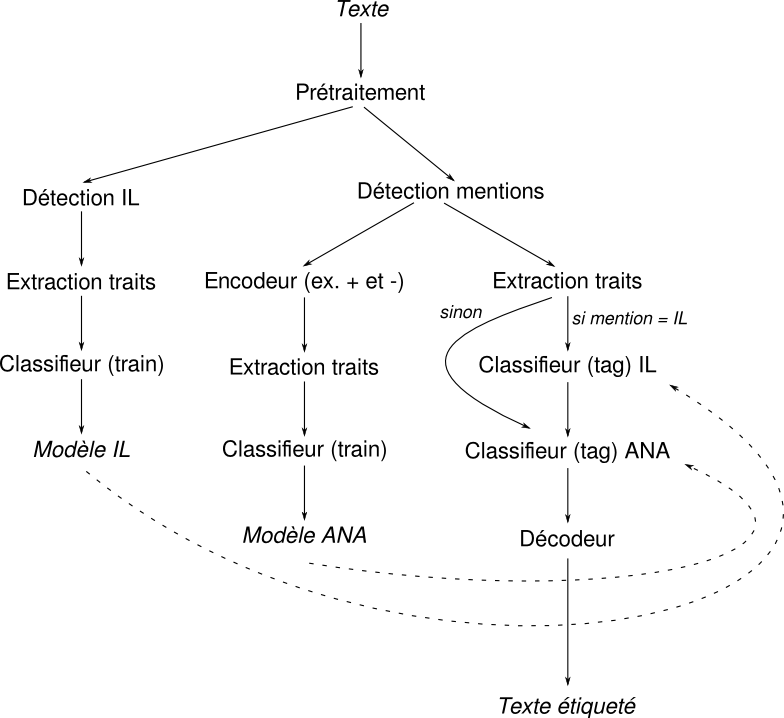
\includegraphics[scale=0.6]{etapes.png}
\end{figure}

\section*{Conclusion}



\bibliographystyle{apalike}
\bibliography{biblio}

\end{document}


%http://people.csail.mit.edu/mcollins/papers/heads